\subsection{ความแตกต่างระหว่างโครงสร้างของมนุษย์กับโครงสร้างของหุ่นยนต์}

\subsubsection{ความแตกต่างขององศาเสรี}
เนื่องจากลักษณะข้อต่อของมนุษย์มีความซับซ้อนมากกว่าโครงสร้างของหุ่นยนต์
ทำให้ข้อต่อแต่ละจุดของมนุษย์นั้นสามารถหมุนได้หลายทิศทาง รวมถึงขอบเขตของการหมุนของข้อต่อในแต่จุดก็มีความแตกต่างกัน
ในการนำรูปแบบการเดินของมนุษย์ไปใช้กับหุ่นยนต์จึงต้องปรับค่ามุมที่ข้อต่อให้มีความเหมาะสมกับโครงสร้าง
และข้อจำกัดเกี่ยวกับการหมุนของข้อต่อจุดต่างๆของหุ่นยนต์ที่จะใช้ทดสอบด้วย

\subsubsection{ความแตกต่างของอัตราส่วน}
นอกจากความแตกต่างขององศาเสรี (DoF) ระหว่างมนุษย์กับหุ่นยนต์แล้ว
ความแตกต่างของอัตราส่วนระหว่างโครงสร้างแต่ละส่วนของมนุษย์กับหุ่นยนต์เป็นอีกสาเหตุหนึ่ง
ที่ต้องทำการปรับแต่งใหม่มีความเหมาะสม เนื่องจากความยาวของโครงสร้างแต่ละส่วน
รวมทั้งระยะห่างระหว่างจุดหมุนแต่ละจุดของมนุษย์กับหุ่นยนต์ที่มีความแตกต่างกัน
ดังนั้นจึงต้องกำหนดระบบพิกัดสำหรับหุ่นยนต์ฮิวมานอยด์ขึ้นมาใหม่ เพื่อใช้ในการอ้างอิงจุดหมุน
และความยาวของโครงสร้างในส่วนต่างๆ
\begin{figure}[!ht]
    \centering
    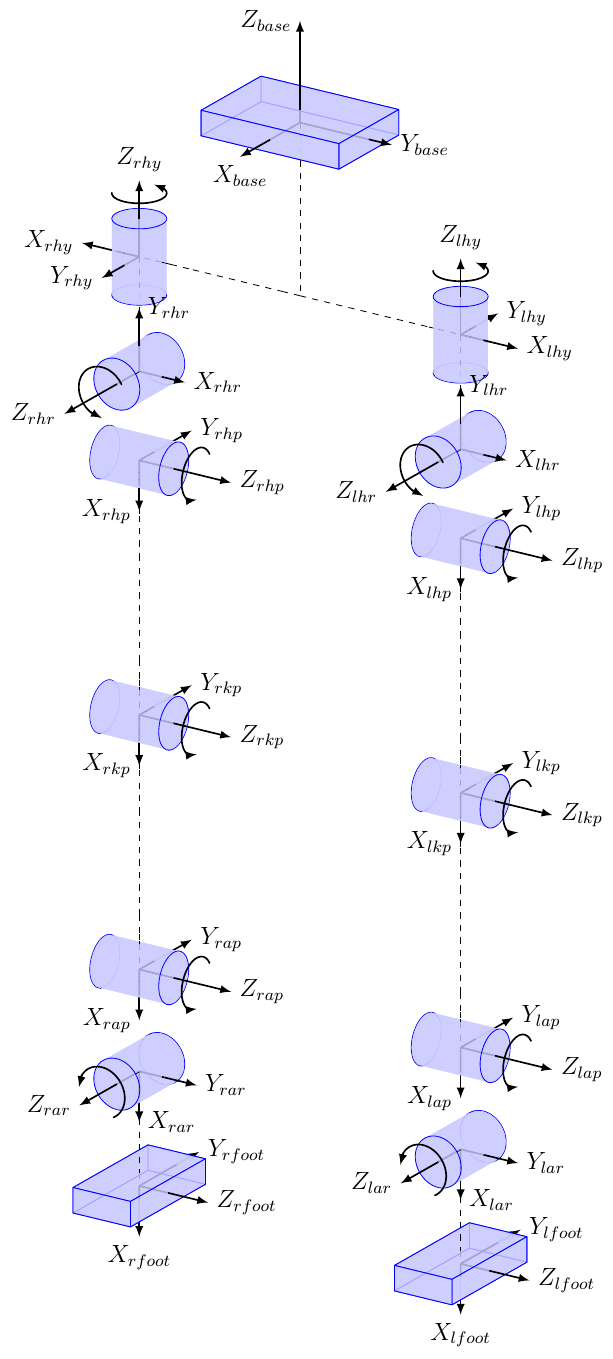
\includegraphics[width=0.40\textwidth]{chapter2/images/uthai_kinematics.png}
    \caption{ตัวอย่างตำแหน่งและการหมุนของข้อต่อของหุ่นยนต์เพื่อการอ้างอิง}
    \label{fig:robot_frame}
\end{figure}

\subsubsection{กำลังและประสิทธิภาพของมอเตอร์}
ความสามารถในการรับน้ำหนักของข้อต่อแต่ละจุดมีความแตกต่างกัน การเคลื่อนไหวของมนุษย์นั้นจะมีกล้ามเนื้อ
และเส้นเอ็นเป็นตัวออกแรงดึงส่วนต่างๆของร่างกายเพื่อทำให้เกิดการเคลื่อนไหวซึ่งจะมีความยืดหยุ่นและแรงดึงที่มีค่าสูง
สำหรับการเคลื่อนไหวของหุ่นยนต์ จะใช้การบิดแกนของเซอร์โวมอเตอร์ (Servo Motor) หรือมอเตอร์ที่ติดอยู่ที่ข้อต่อจุดต่างๆ
ทำให้ความสามารถในการรับน้ำหนัก แรงบิดและความยืดหยุ่นที่ข้อต่อขึ้นกับกำลังของมอเตอร์เป็นหลัก
การสร้างท่าทางของหุ่นยนต์จึงต้องคำนึงถึงความสามารถในการรับน้ำหนักและกำลังของเซอร์โวมอเตอร์ที่ใช้ด้วยเช่นกัน

%%%%%%%%%%%%%%%%%%%%%%%%%%%%%%%%%%%%%%%%%%%%%%%%%%%%%%%%%
%\subsection{วัสดุและการขึ้นรูปโครงสร้างของหุ่นยนต์ฮิวมานอยด์}
%\begin{figure}[ht]
%    \centering
%    
\includegraphics[width=0.40\textwidth]{chapter2/images/toedit.jpg}
%    \caption{รอแก้ไข}
%    \label{fig:toedit}
%\end{figure}

%%%%%%%%%%%%%%%%%%%%%%%%%%%%%%%%%%%%%%%%%%%%%%%%%%%%%%%%%
\subsection{อุปกรณ์ที่ใช้ในหุ่นยนต์ฮิวมานอยด์}

\subsubsection*{ตัวขับเคลื่อน}
ในการสร้างหุ่นยนต์ฮิวมานอยด์นั้นระบบการขับเคลื่อนถือว่าเป็นเรื่องสำคัญ เนื่องจากว่าถ้าหากระบบขับเคลื่อนไม่สามารถทำงานได้อย่างเต็มประสิทธิภาพ
หรือหากมีการออกแบบที่ผิดพลาด จะส่งผลทำให้หุ่นยนต์ฮิวมานอยด์นั้นมีประสิทธิภาพในการทำงานลดลงตามไปด้วย ภายในงานวิจัยนี้ทางผู้จัดทำได้ใช้ตัวขับเคลื่อนเป็น
Dynamixel digital servo EX-106 ซึ่งเป็นเซอร์โวมอเตอร์ที่เหมาะสำหรับทำหุ่นยนต์โดยเฉพาะ ภายในประกอบไปด้วย มอเตอร์กระแสตรง ชุดเฟืองมอเตอร์
ไดรเวอร์คอนโทรเลอร์ สามารถเชื่อมต่อกันผ่าน BUS RS-485 มีการควบคุมแบบ PID และแรงบิดที่สูง\footnote{ Robot Actuator [http://support.robotis.com/en/product/actuator/dynamixel/ex\_series/ex-106.htm] }

\begin{figure}[!ht]
    \centering
    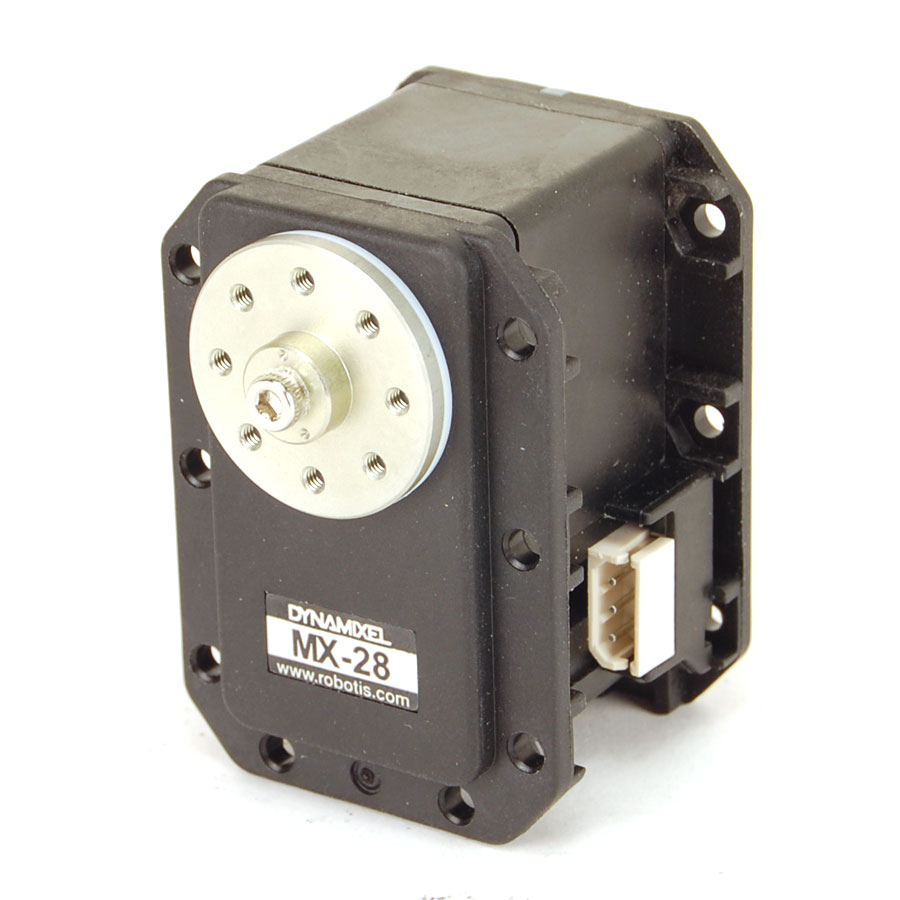
\includegraphics[width=0.3\textwidth]{chapter2/images/actuator_robot.jpg}
    \caption{ตัวขับเคลื่อนที่ใช้ในหุ่นยนต์ฮิวมานอยด์}
    \label{fig:actuator_robot}
\end{figure}

\clearpage
%%%%%%%%%%%%%%%%%%%%%%%%%%%%%%%%%%%%%%%%%%%%%%%%%%%%%%%%%
\subsubsection*{หน่วยประมวลผลควบคุม}
ในการควบคุมหุ่นยนต์ฮิวมานอยด์ให้สามารถทำกิจกรรมต่างๆ คือ
หน่วยประมวลผลระบบควบคุม ถ้าหากไม่มีระบบประมวลผลควบคุมแล้ว อุปกรณ์ต่างๆ ที่ติดตั้งอยู่ภายในตัวของหุ่นยนต์ฮิวมานอยด์จะไม่สามารถติดต่อสื่อสารกันได้
ซอฟท์แวร์ของหุ่นยนต์ที่พัฒนามาทั้งหมดจะไม่สามารถใช้ได้ ทำให้หุ่นยนต์ฮิวมานอยด์ไม่สามารถทำงานในสิ่งที่ต้องการ
การวางแผนระบบควบคุมที่นิยมใช้ในระบบหุ่นยนต์ฮิวมานอยด์ส่วนใหญ่ จะแบ่งออกเป็น 2 ส่วนด้วยกัน 
คือส่วนของหน่วยประมวลผลควบคุมระดับสูง และหน่วยประมวลผลควบคุมระดับต่ำ

\subsubsection*{หน่วยประมวลผลควบคุมระดับสูง (High level controller)}
หน่วยประมวลผลควบคุมระดับสูงเป็นส่วนที่ใช้ประมวลผลการทำงานที่มีความซับซ้อนของระบบเช่น
จลนศาสตร์ของหุ่นยนต์ การคำนวณหาเส้นทางการเดิน ในการคำนวณทางคณิตศาสตร์ของระบบเหล่านี้จำเป็นต้องมีการประมวลผลที่เร็ว
และมีประสิทธิภาพ ในสมัยที่มีการพัฒนาหุ่นยนต์ฮิวมานอยด์ยุคแรกเริ่มนั้น หน่วยประมวลผลควบคุมระดับสูง
จะใช้คอมพิวเตอร์เป็นตัวในการประมวลผลการคำนวณ ซึ่งคอมพิวเตอร์สมัยนั้นมีขนาดใหญ่ น้ำหนักมาก
และต้องใช้หลังงานสูง ซึ่งต่างจากปัจจุบันนี้ที่มีการพัฒนาของเทคโนโลยีที่ก้าวหน้ามากขึ้น
ทำให้คอมพิวเตอร์มีขนาดเล็กลงเทียบเท่ากับบอร์ดคอนโทรเลอร์ทั่วไป\footnote{Robot controller Robotis, Thormang, http://jp.robotis.com/index/product.php?cate\_code=111410}

\begin{figure}[!ht]
    \centering
    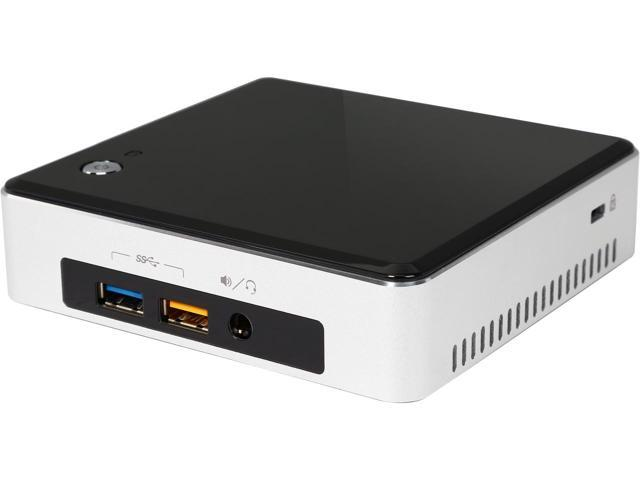
\includegraphics[width=0.3\textwidth]{chapter2/images/thormang_controller.jpg}
    \caption{ตัวประมวลผลระดับสูงของ Thormang Humanoid}
    \label{fig:thormang_controller}
\end{figure}

\subsubsection*{หน่วยประมวลผลควบคุมระดับต่ำ (Low level controller)}
หน่วยประมวลผลควบคุมระดับต่ำเป็นส่วนที่รับคำสั่งมาจากหน่วยประมวลผลควบคุมระดับสูง
มีประสิทธิภาพในการประมวลผลการคำนวณที่น้อยกว่า เนื่องจากการออกแบบสถาปัตยกรรมภายในระบบไม่เอื้ออำนวยต่อการคำนวณที่มีความซับซ้อน
แต่มีความสามารถในการประมวลผลระบบที่เป็นคาบได้อย่างแม่นยำ ในด้านการทำหุ่นยนต์ฮิวมานอยด์นั้นมักจะใช้หน่วยประมวลผลควบคุมระดับต่ำ
ในการติดต่อกับอุปกรณ์ต่างๆบนตัวของหุ่นยนต์ฮิวมานอยด์โดยตรง เช่น ตัวขับเคลื่อน เซนเซอร์รับค่า หรือไฟแสดงสถานะต่างๆของหุ่นยนต์
\begin{figure}[!ht]
    \centering
    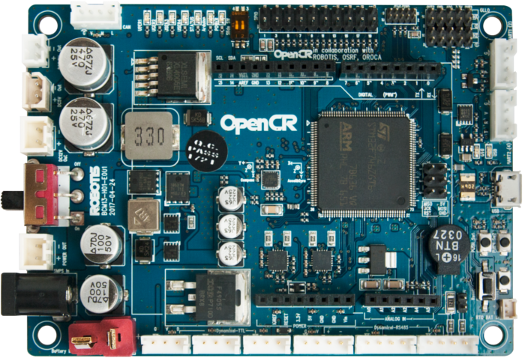
\includegraphics[width=0.30\textwidth]{chapter2/images/opencr_op3.png}
    \caption{ตัวประมวลผลระดับต่ำของ Robotis OP3 Humanoid}
    \label{fig:opencr_op3_controller}
\end{figure}

\clearpage
%%%%%%%%%%%%%%%%%%%%%%%%%%%%%%%%%%%%%%%%%%%%%%%%%%%%%%%%%
\subsubsection*{เซนเซอร์ตรวจหน้าสัมผัสที่พื้น}
เซนเซอร์ตรวจหน้าสัมผัสที่พื้นเป็นเซนเซอร์ที่ถูกติดตั้งบริเวณฝ่าเท้า เพื่อตรวจสอบการเดินของหุ่นยนต์ฮิวมานอยด์ว่าขณะนี้มีการสัมผัสของฝ่าเท้าของหุ่นยนต์กับพื้นหรือไม่
ซึ่งในงานวิจัยนี้ได้ใช้หลักการตัวตรวจจับแรงกดแบบค่าความต้านทานหรือ Force Sensing Resistor (FSR)\footnote{ [UNICON] Force sensor with UNICON [http://doc.inex.co.th/force-sensor-with-unicon/] }
ที่ใช้เทคโนโลยีฟิล์มโพลีเมอร์แบบหนาโดยที่
เซนเซอร์สามารถเปลี่ยนแรงที่มากระทำให้อยู่ในรูปของการเปลี่ยนแปลงค่าความต้านทานไฟฟ้า ตัวเซนเซอร์มีลักษณะเป็นแผ่น มีโครงสร้าง 5 ชั้น
โดยสองชั้นนอกสุดเป็นฟิล์มของโพลีเอสเตอร์ สองชั้นถัดเข้ามาเป็นฟิล์มของโลหะที่เป็นตัวนำไฟฟ้า และชั้นในสุดเป็นหมึกที่มีความไวในการตอบสนองต่อแรงภายนอกที่มากระทำ
(Pressure sensitive ink) และโครงสร้างทั้ง 5 ชั้น ถูกรวมเข้าด้วยกันด้วยวิธีลามิเนท จึงทำให้เซนเซอร์วัดแรงนี้มีลักษณะแบนมีความยืดหยุ่นสูง
ด้วยเหตุนี้จึงทำให้เซนเซอร์สามารถโค้งงอได้ง่าย แรงดันไฟฟ้าที่ตกคร่อมตัวตรวจจับจะลดลง เมื่อมีแรงกดมากระทำบนแผ่นตรวจจับ มีโครงสร้างของตัวตรวจจับแสดงในรูปที่ \ref{fig:fsr_sensor} 

\begin{figure}[!ht]
    \centering
    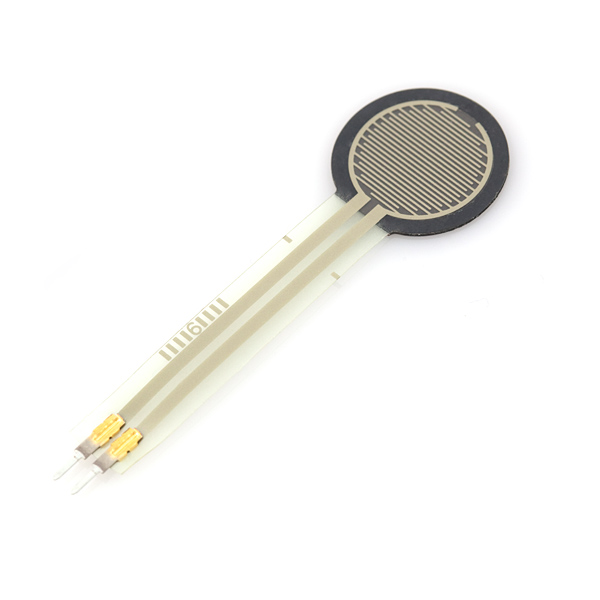
\includegraphics[width=0.15\textwidth]{chapter2/images/FSRx.jpg}
    \caption{ลักษณะโครงสร้างของตัวตรวจจับแรงกด FSR}
    \label{fig:fsr_sensor}
\end{figure}

\subsubsection*{เซนเซอร์วัดความเฉื่อย}
Inertial Measurement Unit (IMU) เป็นส่วนประกอบหลักที่ใช่ในการนำร่องเครื่องบิน ยาน-อวกาศ ดาวเทียม เรือ
ขีปนาวุธ ซึ่งในตัวของ IMU ประกอบไปด้วยสองส่วนหลักคือ Accelerometers 3 ทิศทาง ในการรับความเร่งเชิงเส้น
และ Gyroscopes 3 ทิศทาง ในการบอกความเร็วเชิงมุม เซนเซอร์ตัวนี้สามารถนำมาใช้ในการหาทิศทางการหมุนของตัวหุ่นยนต์ฮิวมานอยด์ได้

เซนเซอร์วัดความเร็ว (Gyroscope)\footnote{ Mechanic gyroscope two-degree of freedom [https://www.bosch-sensortec.com/bst/products/motion/gyroscope/overview\_gyroscopesensors] }
เป็นอุปกรณ์สำหรับการวัดความเร็ว หรือการรักษาการปรับทิศทาง ขึ้นอยู่กับหลักการของการอนุรักษ์โมเมนตัมเชิงมุม
ถ้าไม่มีการเคลื่อนที่ อัตราการเปลี่ยนแปลงมุมจะมีค่าเท่ากับศูนย์

เซนเซอร์วัดความเร่ง (Accelerometer)\footnote{ Accelerometer and Gyroscopes Sensor [https://www.maximintegrated.com/en/app-notes/index.mvp/id/5830] }
เป็นอุปกรณ์ที่ใช้วัดความเร่งเชิงเส้น โดยอาศัยการวัดแรงที่กระทำต่อน้ำหนัก
อ้างอิงที่เกิดจากแรงโน้มถ่วงโลก ซึ่งแรงโน้มถ่วงของโลกจะเป็นเวกเตอร์ชี้ไปที่แกนกลางโลกเสมอ ตามกฎของนิวตัน
\begin{figure}[!ht]
    \centering
    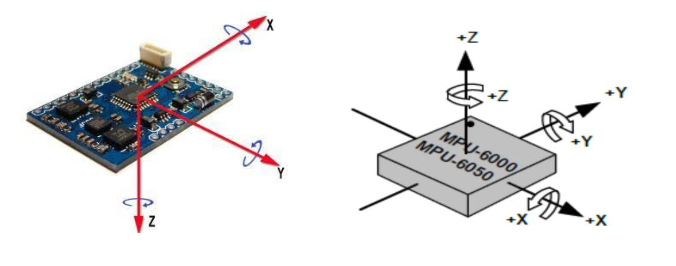
\includegraphics[width=0.5\textwidth]{chapter2/images/imu.png}
    \caption{เซนเซอร์วัดความเฉื่อย}
    \label{fig:imu_sensor}
\end{figure}

%\clearpage
%\subsection{แนวคิดการออกแบบกลไกการเดินของหุ่นยนต์ฮิวมานอยด์}
%การออกแบบหุนยนตฮิวมานอยด์ใหสามารถเดินสองขาไดเสมือนมนุษยโดยใชจํานวนองศาอิสระใหเท่ากับมนุษยนั้นพบวา
%มีขอจํากัดทางดานการออกแบบอยู่มาก เนื่องมาจากอุปกรณที่ใชในการขับเคลื่อนขอตอตางๆ มีอยูอยางจํากัด
%รวมถึงขอจํากัดทางดานตัวรับรูตัวขับของหุนยนต ดังนั้นผูจัดทําจึงออกแบบหุนยนตใหมีองศาอิสระของขอตอ ในขาหนึ่งขาง
%เทากับหกองศาอิสระ ทั้งนี้หุนยนตยังสามารถเคลื่อนที่ไดในปริภูมิ และองศาอิสระเพียงพอตอการใชงาน